% !TEX root = ../my-thesis.tex
%
\chapter{Discussion}\label{sec:discussion}
After the calculation of the models, the next step is to critically examine and evaluate the results. The evaluation of the spatial models follows a simple scheme. First, a brief look is taken at the models without the spatial component, before the spatial models are reviewed and compared with the non-spatial models. Next, it is examined which factors significantly influence the risk of infection and why these factors might have an impact. For this, the coefficient of the BYM2 model are analysed. Finally, a look at area-specific risk is taken to see which regions in a given country are most at risk.
\section{Discussion of the (Non)-Temporal Models}
\subsection{Discussion of the (Non)-Temporal Models for Norway}\label{sec:models_norway}
The non-spatial model for Norway identifies five significant effects:
\begin{itemize}
    \item The number of unemployed immigrants 
    \item The total number of immigrants 
    \item The urban density 
    \item The proportion of females 
\end{itemize}
Moreover, the intercept is significant. \\
Comparing the spatial models with the non-spatial models using Table~\ref{allNorway}, it can be seen that BYM2, Besag and the non-spatial model perform almost equally well in terms of the DIC and WAIC, while the Leroux model performs best in terms of these two metrics. In terms of CPO, all spatial models perform better than the non-spatial model, with the Leroux model again performing best. However, the MAE shows that the non-spatial model has the best predictive performance, ahead of the Besag model, the BYM2 model and the Leroux model. This shows that the Leroux model overfits the training data more than the other models, a characteristic that can be seen in Figure~\ref{comparison_norway_1}. The fact that the non-spatial model performs better than the spatial models is an indication that the spatial effect in Norway is not strong and that a different class of models may be better suited to identify critical factors affecting infection rates. Table~\ref{fixedAllNorway_spatial} shows that adding the spatial effect did not suddenly cause any variables to become significant, while all variables, including the intercept, that are significant in the non-spatial model remain significant. Nevertheless, significant effects are found and have to be discussed. \\
The exponentiated intercept implies a risk rate of -59.1\% across Norway. Factors related to immigration play a crucial role in the relative risk of developing Covid-19. A one standard deviation increase in the number of unemployed immigrants leads to a 22.6\% increase in risk and a one standard deviation increase in the total number of immigrants leads to a 22.8\% increase in risk. Unfortunately, there are no studies analysing the relationship between unemployed immigrants and the risk of developing Covid-19, as studies mostly focus on the relationship between unemployment in general and the risk of disease. Unemployment, however, turns out to be non-significant in the BYM2 model. Looking at older studies, Elkeles and Seifert (1996) conducted a longitudinal study that looked at the unemployment status and health of labour migrants in Germany. They found that immigrants are often employed in jobs with higher health risks and stress and therefore had poorer health \autocite[][]{elkeles1996immigrants}. Sia et al. (2019) analysed the association between immigration status and unemployment and men's and women's health using data from the Canadian Health Measures Survey. The study provided evidence of biological associations between unemployment and the likelihood of common chronic diseases, inflammation and possible malnutrition, with unemployed immigrants, and particularly unemployed immigrant women, being more prone to chronic diseases \autocite[][]{sia2019chronic}. Thus, there is precedent for an association between unemployment and immigrants and a higher risk of disease, however, further research would need to be conducted to analyse the association between unemployed immigrants and the risk of Covid-19 infection. \\
The last factor that influences the relative risk is urban density, where an increase of 1 standard deviation leads to an increase in the relative risk of 20.1\%. The relationship between a higher number of residential buildings in a given area and the number of infections is probably due to the fact that with an increasing number of residential buildings comes an increasing number of inhabitants. A look at the Bravais-Pearson correlation coefficient confirms this assumption with $\rho=0.7070$. Furthermore, the correlation between urban density and population density is $0.8037$. This is convenient since studies analysing the relationship between urban density and Covid-19 usually define urban density as the number of inhabitants per square kilometre. Because of the positive relationship between urban density and population density, urban density acts as a proxy for population density in these models, so the relationship between higher population density and higher case numbers should account for the higher infection rates in areas with higher urban density. According to Jamshidi et al. (2020) and Whittle \& Diaz-Artiles (2020), higher urban/population density and higher infection numbers are due to a decrease in proximity between people and an increase in the likelihood of interpersonal contact \autocite[][]{jamshidi2020global, whittle2020ecological}. Sigler et al. (2020) found that dense urban environments provide more opportunities for the virus to spread, but that higher density had a stronger effect earlier and decreased in strength and importance over time\autocite[][]{sigler2020socio}. \\
A higher risk among immigrants in Norway is found in a study by Indseth et al. (2020). The reasons given are barriers to adequate information due to low health literacy in certain groups and misconceptions about Covid-19 or test criteria, as well as other socio-economic and environmental factors \autocite[][]{indseth2020covid}. Therefore, the results of the BYM2 model are consistent with this study. \\
Looking at the factors that reduce the risk of infection for Covid-19, a 1 standard deviation increase in the proportion of women leads to an 18.9\% reduction in the risk of infection. This result is not consistent with current research.  Many studies have investigated the relationship between gender and Covid-19 and most come to the same conclusion. While the risk of infection is the same in men and women, men tend to experience a higher severity and mortality rate for Covid-19 compared to women \autocite[][]{mukherjee2021covid, gausman2020sex, spagnolo2020sex, kopel2020racial}. \\
A look at the relative risk of infection in Figure~\ref{rr_norway} shows that the relative risk is below 1 in most of Norway, which is not too surprising considering that Norway has managed the pandemic quite well so far. The two municipalities with the highest relative risk are Iveland and Ålesund. However, a look at the posterior probability in Figure~\ref{posterior_norway} shows that the posterior probability of the risk being greater than 1 is around 0.5 for Ålesund (0.503) and less than 0.75 for Iveland (0.640). Looking at the log posterior mean of the random effects, there is an increased risk in the regions around Oslo and in large parts of southern and central Norway, while the risk tends to be lower in the northern parts of the country.
\begin{figure}[H]
  \centering
  \includegraphics[width = \textwidth]{relative_risk_norway.png}
  \caption{Relative risk of contracting Covid-19 in Norway.}
  \label{rr_norway}
\end{figure}
\begin{figure}[H]
  \centering
  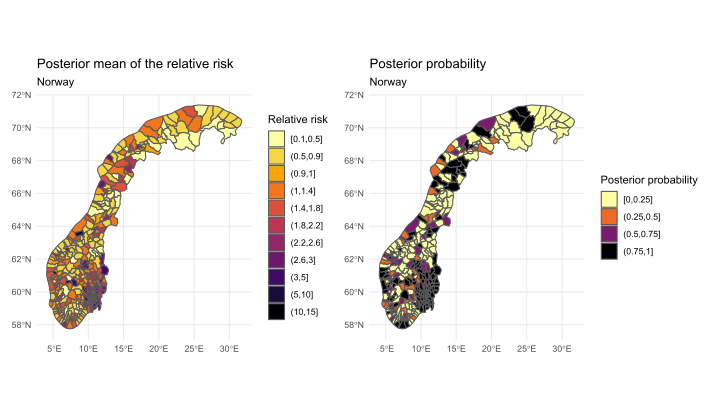
\includegraphics[width = \textwidth]{posterior_norway.png}
  \caption{Posterior mean of the municipality-specific relative risks $\zeta=\exp{\left(\xi\right)}$ compared with the whole of Norway (left) and posterior probability $\mathbb{P}\left(\zeta_i>1|\pmb{y}\right)$}
  \label{posterior_norway}
\end{figure}
\subsection{Discussion of the (Non)-Temporal Models for Germany}
In the non-spatial model for Germany, six coefficients are significant, in addition to the intercept:
\begin{itemize}
    \item The percentage of the vote for the right-wing populist AfD
    \item The population density
    \item The logarithmic trade tax
    \item The percentage of the vote for the SPD
    \item The percentage of the vote for the left-wing party "Die Linke"
    \item The percentage of the vote for the Green party
\end{itemize}
A look at Table~\ref{allGermany} shows that the spatial models outperform the non-spatial model in terms of the DIC and the WAIC, while all models perform about equally well in terms of the CPO. The predictive performance is best for the BYM2 model, just ahead of the Besag model, as indicated by the lowest values for the MAE. When adding the spatial term for the BYM2 model, several variables lose their significance, namely the percentage of the vote for the SPD, "Die Linke" and the Greens, while the intercept, the percentage of the vote for the AfD, population density and the logarithmic trade tax remain significant. \\
The exponentiated intercept implies a risk rate of -6.8\% across Germany. The greatest influence on the relative risk is determined to be the percentage of the vote for the far-right AfD. An increase in this variable by 1 standard deviation leads to an increase in the relative risk by 25.7\%. The AfD openly criticizes the measures taken by the government in Germany to prevent the spread of Covid-19, which leads to a large proportion of the party's voters not taking the measures seriously and refusing to keep a safe distance or wear a mask in public spaces. Several studies have taken a look at the response of right-wing parties to the pandemic and how people who vote for these types of parties have reacted. Wondreys and Mudde (2020) point out that these parties were quick to warn about the virus, but once cases spiked, they criticized the measures taken to contain the spread of the virus. They noted that right-wing parties often rejected the measures proposed by the leading parties because they themselves are part of the opposition \autocite[][]{wondreys2020victims}, as is the case with the AfD in Germany. Vieten (2020) shows how the far-right mobilizes people for anti-hygiene or anti-lockdown protests and how this is used to normalize the global far-right \autocite[][]{vieten2020new}. Eberl et al. (2020) analysed data from the Austrian Corona Panel Project to test whether populism attitudes and belief in conspiracy theories related to Covid-19 are correlated. Using structural equation modelling, they show that populism indirectly influences Covid-19 conspiracy beliefs through trust in political and scientific institutions. They find that populist attitudes have a negative correlation with trust in the government and the parliament.Furthermore, they find that higher populist attitudes are negatively correlated with trust in science, a factor that reduces belief in Covid-19 conspiracy theories \autocite[][]{eberl2020populism}. Finally, Farias and Pilati (2020) conducted a study in Brazil to predict social distancing violation intention and past non-compliance during the Covid-19 pandemic, controlling for the effects of interolerence of insecurity and socio-demographic variables. Their results included that individuals who support right-wing parties are more likely to violate social distancing measures \autocite[][]{farias2020violating}. \\
An increase in population density by 1 standard deviation leads to a risk increase of 10.9\%. Reasons why a higher population density correlates positively with the number of infections are discussed in Section~\ref{sec:models_norway}. \\
The last significant effect is the logarithmic trade tax with an increase of 1 standard deviation leading to a 6.8\% increase in risk. There are no studies that specifically analyse the relationship between the trade tax and the risk of infection, but some studies have analysed infection rates in different spatial areas while controlling for factors such as income. In general, a negative relationship is found between areas with higher income and infection rates, meaning that areas with higher income had fewer cases of Covid-19. Cordes and Castro (2020) found that postcode areas in New York City with a low proportion of positive tests had higher incomes and tested less compared to lower income areas. They found that people in lower income areas are more likely to be without health insurance \autocite[][]{cordes2020spatial}. Coven and Gupta (2020) found that New York City residents who come from wealthier neighbourhoods are more likely to flee the city, and that people who live in low-income neighbourhoods are more likely to have frontline occupations and visit retail shops more often, increasing their exposure to Covid-19 \autocite[][]{coven2020disparities}. The situation seems to be the same in Europe, as Baena et al. (2020) found that districts in Barcelona with a lower average income had a higher Covid-19 incidence. They found that the incidence in the district with the lowest income is 2.5 times higher than in the district with the highest income \autocite[][]{baena2020impact}. Again, the results of the BYM2 model are not consistent with current research. \\
The relative risk of infection shown in Figure~\ref{rr_germany} is highest in Eastern Germany, more specifically in the federal state of Saxony. Saxony has established itself as the political stronghold of the AfD in recent years, which has even led to the ruling party, the Union, moving further to the right on the political spectrum. In addition to Saxony, the traditionally highly conservative Bavaria and the populous Ruhr region have a relative risk of over 1. Figure~\ref{posterior_germany} shows that for most of these regions the posterior mean of the random effects is over 1, mostly with a posterior probability of at least 0.75.
\begin{figure}[H]
  \centering
  \includegraphics[width = \textwidth]{relative_risk_germany.png}
  \caption{Relative risk of contracting Covid-19 in Germany.}
  \label{rr_germany}
\end{figure}
\begin{figure}[H]
  \centering
  \includegraphics[width = \textwidth]{posterior_germany.png}
  \caption{Posterior mean of the municipality-specific relative risks $\zeta=\exp{\left(\xi\right)}$ compared with the whole of Germany (left) and posterior probability $\mathbb{P}\left(\zeta_i>1|\pmb{y}\right)$}
  \label{posterior_germany}
\end{figure}
\subsection{Comparison Between the Spatial Models and the Predictive Models}
Looking at the predictive models again and comparing them to the spatial models, both Table~\ref{pred_perf} and Table~\ref{pred_perf_norway} show that the predictive models perform significantly worse than the spatial models. For Germany, the test MAE of the random forest is about 80\% higher than that of the BYM2 model, while in Norway it is about 50\% higher. This could indicate that the spatial effect in Norway is not as strong as in Germany, mainly due to the fact that most of the cases in Norway are located in Oslo and the surrounding municipalities. However, the smaller relative difference could be due to the fact that the infection numbers in Norway are significantly lower than in Germany, which naturally leads to a smaller mean absolute error. Nevertheless, the comparison between the two model classes is interesting, as different features turn out to be important for both countries, compared to the BYM2 model for each country. For Germany, it is the number of clinics, the number of public transport platforms and the number of marketplaces, while for Norway it is the number of places of worship, the number of offices, the number of public transport platforms and the number of colleges and universities. For Germany, the logarithmic business tax is the only feature that is important in both models, while for Norway, urban density is the only feature that is important in the BYM2 model and the random forest. \\
Most interesting here, however, is that in both countries the number of public transport platforms is an important factor in explaining infection rates in a municipality. The association between the risk of Covid-19 infection and public transport is well studied. Hu et al. (2021) conducted a study in which they analysed the risk of transmission of the disease on high-speed trains in China. To do this, they used data from around 2300 patients and 72,000 close contacts who had a travel time between 0 and 8 hours from 19 December 2019 to 6 March 2020. They analysed the spatial and temporal distribution of Covid-19 transmission among train passengers to identify associations between infection, spatial distance and travel time. They found a high risk of transmission among train passengers, which showed significant differences depending on travel time and seat position. They suggest reducing the risk of transmission by increasing seat pitch, reducing passenger density and using hygiene equipment \autocite[][]{hu2021risk}. Musselwhite (2020) compares Covid-19 with other infectious diseases that may have similar properties, noting that other types of human coronavirus, e.g. SARS coronavirus or MERS coronavirus, can survive on inanimate surfaces such as metal, glass or plastic for up to nine days and similar surface stability has been observed for SARS-CoV-2. In addition, a link has already been observed between acute respiratory infection (ARI) in winter and the use of buses or trams in the five days before the onset of symptoms. Finally, the greatest risk for infectious diseases on public transport is proximity between people in an enclosed environment. If people do not close their mouths when coughing and sneezing, public transport can become a significant source of microorganisms \autocite[][]{musselwhite2020editorial}.
\clearpage
\section{Discussion of the Temporal Models}
The temporal models for Germany and Norway do not perform as well as hoped. One of the problems for the models is that no distribution is found that fits the data reasonably well. In the end, a negative binomial distribution is used because it seems to fit slightly better than a normal distribution. Especially the QQ-plots in Figure~\ref{fitNegbinomGermany_ts} and Figure~\ref{fitNegbinomNorway_ts} illustrate this problem. The models themselves do not show an unreasonably high value for the MAE of the test data, but this is mainly due to the fact that the test set is kept relatively small with only 20 observations. Table~\ref{germany_temporal_2} shows what happens when the test size for the temporal models for Germany is increased. The MAE in training remains surprisingly low, but the test MAE increases exponentially as the test size increases. 
\begin{table}[H] 
\caption{The performance measures for different types of temporal models for Germany. \label{germany_temporal_2}}
\begin{tabular}{l r r r r r}
\toprule
\textbf{Model}	& Test size & \textbf{$\hbox{MAE}_{\hbox{train}}$} & \textbf{$\hbox{MAE}_{\hbox{test}}$}\ \\
\midrule
Only date as covariate & 20 & 4915 & 27450 \\
Random walk of second order & 20 & 2009 & 6180 \\
AR(1) process & 20 & 18 & 7524 \\
Temporal model &  20 & 1931 & 5821 \\
Only date as covariate & 40 & 4782 & 22559 \\
Random walk of second order & 40 & 1832 & 2090247 \\
AR(1) process & 40 & 7 & 26561 \\
Temporal model &  40 & 1764 & 10457609 \\
Only date as covariate & 60 & 4597 & 22525 \\
Random walk of second order & 60 & 1656 & 5.81e+12 \\
AR(1) process & 60 & 8 & 99471 \\
Temporal model &  60 & 1584 & 5.09e+16 \\
\bottomrule
\end{tabular}
\end{table}
The same effect can be observed for Norway. Even with the small test size, which leads to a low mean absolute error of the test, the quality of the prediction in Germany is not as high, since according to the prognosis the number of infections increases, while in reality the number of infections in Germany decreases. This is illustrated by the comparison between the predicted 7-day incidence and the actual 7-day incidence in Figure~\ref{incidence_germany}, which shows an increase in the predicted 7-day incidence, while in reality the incidence decreases rapidly. For Norway, the comparison between incidences is slightly better, as at least for the last days of the test set, the predicted incidence and the actual incidence both increase as can be seen in Figure~\ref{incidence_norway}. \\
Finally, despite trying a variety of models during this work, hardly any coefficient turned out to be significant and interpretable, as often significant coefficients had values in the tens of thousands. In the models that are ultimately used in this work, the only significant feature besides the intercept turned out to be workplace mobility, with a one standard deviation increase in the mobility leading to a risk increase of 18.6\% in Germany and 20.1\% in Norway. \\
Studies on indoor infection risk are numerous and mostly point to the same thing, namely that aerosols from infected people can effectively transmit the virus indoors. Measures such as wearing face masks and ventilating rooms can reduce the risk of infection, but the most effective measure is still not going to the workplace \autocite[][]{lelieveld2020model, bedford2020covid, hall2020covid}.